\chapter{Domain modeling process}

In our thesis, we consider a domain modeling process stating with a domain description $T$ acquired from stakeholders and knowledge sources such as internal documentation, manuals, or state law. $T$ can be a well-curated text, but may also encompass varied interpretations articulated by different stakeholders at various levels of detail. A modeling expert translates $T$ into a domain model $M$ in a sequence of steps.

A domain model $M = (\mathcal{C}, \mathcal{P})$ consists of a set of classes $\mathcal{C}$ and properties $\mathcal{P}$.

A class $C \in \mathcal{C}$ has its $name(C)$ which identifies $C$ in $M$ and briefly characterizes the semantics of $C$. The class $C$ also has a $description(C)$ that describes the semantics of $C$.

A Property $P \in \mathcal{P}$ has also $name(P)$ and $description(P)$ used for the same purposes. It has a $cardinality(P)$ that refers to the specification of the number of instances of one class that can or must be associated with each instance of another class. It also has a source class, such that $source(P) \in \mathcal{C}$ and it can have a target class such that $target(P) \in \mathcal{C}$. $P$ is a binary association if $target(P)$ is defined otherwise, $P$ is an attribute.

These basic modeling constructs are prevalent in real conceptual models \cite{Keet2015}, so their automation could have a significant impact. We distinguish the following steps.


\section{Steps}

\textbf{Design a class}:
for a concept in $T$, create a class $C$ with a designated $name(C)$.

\textbf{Design an attribute for a class}:
for a class $C$ and a concept in $T$ that characterizes $C$, create an attribute $P$, where $C = source(P)$, and define its $name(P)$.

\textbf{Design an association for a class}:
for a class $C$ and a concept in $T$ that describes a relationship of $C$ with another concept, create an association $P$ such that $C = source(P)$ or $C = target(P)$, and define its $name(P)$. If not yet represented, create a class $D$ for the other concept and specify its $name(D)$.

\textbf{Design a description for a class}:
for a class $C$ and a concept in $T$ that describes $C$, define $description(C)$

\textbf{Design a description for an attribute}:
for an attribute $P$ and a concept in $T$ that describes $P$, define $description(P)$

\textbf{Design a description for an association}:
for an association $P$ and a concept in $T$ that describes $P$, define $description(P)$

\textbf{Design a data type for an attribute}:
for an attribute $P$ and a concept in $T$ that describes $P$, define $dataType(P)$

\textbf{Design a cardinality for an attribute}:
for an attribute $P$ and a concept in $T$ that describes $P$, define $cardinality(P)$

\textbf{Design a cardinality for an association}:
for an association $P$ and a concept in $T$ that describes $P$, define $cardinality(P)$


\section{Example}

Consider the domain model in figure \ref{fig:modeling-steps}. It contains a class ``employee'' with attribute ``name'' and with association ``works in'' with the class ``Department''.

\begin{figure}[!h]
    \centering
    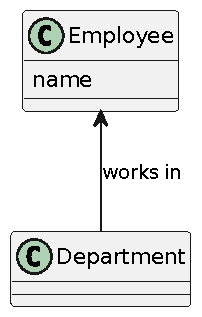
\includegraphics[scale=1.00]{img/domain-modeling-steps-example.pdf}
    \caption{\centering Simple domain model example}
    \label{fig:modeling-steps}
\end{figure}

To create this domain model when starting from an empty domain model we can for example execute the following steps:

\begin{enumerate}
\item design a class ``employee''
\item design a class ``department''
\item design an attribute ``name'' for a class ``employee''
\item design an association ``works in'' for a class ``employee'' and ``department''
\end{enumerate}

For providing more information for this domain model we can use the mentioned steps for defining description of the modeled elements, for defining data type of the modeled attributes and for defining cardinalities of the modeled attributes and associations.